\documentclass[a4paper]{article}

\usepackage{inputenc}
\usepackage[british,UKenglish]{babel}
\usepackage{amsmath}
%\usepackage{titlesec}
\usepackage{color}
\usepackage{graphicx}
\usepackage{fancyref}
\usepackage{hyperref}
\usepackage{float}
\usepackage{scrextend}
\usepackage{setspace}
\usepackage{xargs}
\usepackage{multicol}
\usepackage{nameref}

\usepackage{sectsty}
\usepackage{multicol}
\usepackage{multirow}
\usepackage[procnames]{listings}
\usepackage{appendix}

\newcommand\tab[1][1cm]{\hspace*{#1}}
\hypersetup{colorlinks=true, linkcolor=black}
\interfootnotelinepenalty=10000

\newcommand{\cleancode}[1]{\begin{addmargin}[3em]{3em}\texttt{\textcolor{cleanOrange}{#1}}\end{addmargin}}
\newcommand{\cleanstyle}[1]{\text{\textcolor{cleanOrange}{\texttt{#1}}}}


\usepackage[colorinlistoftodos,prependcaption,textsize=footnotesize]{todonotes}
\newcommandx{\commred}[2][1=]{\textcolor{Red}
{\todo[linecolor=red,backgroundcolor=red!25,bordercolor=red,#1]{#2}}}
\newcommandx{\commblue}[2][1=]{\textcolor{Blue}
{\todo[linecolor=blue,backgroundcolor=blue!25,bordercolor=blue,#1]{#2}}}
\newcommandx{\commgreen}[2][1=]{\textcolor{OliveGreen}{\todo[linecolor=OliveGreen,backgroundcolor=OliveGreen!25,bordercolor=OliveGreen,#1]{#2}}}
\newcommandx{\commpurp}[2][1=]{\textcolor{Plum}{\todo[linecolor=Plum,backgroundcolor=Plum!25,bordercolor=Plum,#1]{#2}}}

\def\code#1{{\tt #1}}

\def\note#1{\noindent{\bf [Note: #1]}}

\makeatletter
%% The "\@seccntformat" command is an auxiliary command
%% (see pp. 26f. of 'The LaTeX Companion,' 2nd. ed.)
\def\@seccntformat#1{\@ifundefined{#1@cntformat}%
   {\csname the#1\endcsname\quad}  % default
   {\csname #1@cntformat\endcsname}% enable individual control
}
\let\oldappendix\appendix %% save current definition of \appendix
\renewcommand\appendix{%
    \oldappendix
    \newcommand{\section@cntformat}{\appendixname~\thesection\quad}
}
\makeatother


% "define" Scala
\usepackage[T1]{fontenc}  
\usepackage[scaled=0.82]{beramono}  
\usepackage{microtype} 

\sbox0{\small\ttfamily A}
\edef\mybasewidth{\the\wd0 }

\lstdefinelanguage{scala}{
  morekeywords={abstract,case,catch,class,def,%
    do,else,extends,false,final,finally,%
    for,if,implicit,import,match,mixin,%
    new,null,object,override,package,%
    private,protected,requires,return,sealed,%
    super,this,throw,trait,true,try,%
    type,val,var,while,with,yield},
  sensitive=true,
  morecomment=[l]{//},
  morecomment=[n]{/*}{*/},
  morestring=[b]",
  morestring=[b]',
  morestring=[b]"""
}

\usepackage{color}
\definecolor{dkgreen}{rgb}{0,0.6,0}
\definecolor{gray}{rgb}{0.5,0.5,0.5}
\definecolor{mauve}{rgb}{0.58,0,0.82}

% Default settings for code listings
\lstset{frame=tb,
  language=scala,
  aboveskip=3mm,
  belowskip=3mm,
  showstringspaces=false,
  columns=fixed, % basewidth=\mybasewidth,
  basicstyle={\small\ttfamily},
  numbers=none,
  numberstyle=\footnotesize\color{gray},
  % identifierstyle=\color{red},
  keywordstyle=\color{blue},
  commentstyle=\color{dkgreen},
  stringstyle=\color{mauve},
  frame=single,
  breaklines=true,
  breakatwhitespace=true,
  procnamekeys={def, val, var, class, trait, object, extends},
  procnamestyle=\ttfamily\color{red},
  tabsize=2
}

\lstnewenvironment{scala}[1][]
{\lstset{language=scala,#1}}
{}
\lstnewenvironment{cpp}[1][]
{\lstset{language=C++,#1}}
{}
\lstnewenvironment{bash}[1][]
{\lstset{language=bash,#1}}
{}
\lstnewenvironment{verilog}[1][]
{\lstset{language=verilog,#1}}
{}



%代码段设置
\lstset{numbers=left,
basicstyle=\tiny,
numberstyle=\tiny,
keywordstyle=\color{blue!70},
commentstyle=\color{red!50!green!50!blue!50},
frame=single, rulesepcolor=\color{red!20!green!20!blue!20},
escapeinside=``
}

\graphicspath{ {figures/} }
\usepackage{ctex}
\usepackage{graphicx}
\usepackage{color,framed}%文本框
\usepackage{listings}
\usepackage{caption}
\usepackage{amssymb}
\usepackage{enumerate}
\usepackage{xcolor}
\usepackage{bm} 
\usepackage{lastpage}%获得总页数
\usepackage{fancyhdr}
\usepackage{tabularx}  
\usepackage{geometry}
\usepackage{minted}
\usepackage{graphics}
\usepackage{subfigure}
\usepackage{float}
\usepackage{pdfpages}
\usepackage{pgfplots}
\pgfplotsset{width=10cm,compat=1.9}
\usepackage{multirow}
\usepackage{footnote}
\usepackage{booktabs}

%-----------------------伪代码------------------
\usepackage{algorithm}  
\usepackage{algorithmicx}  
\usepackage{algpseudocode}  
\floatname{algorithm}{Algorithm}  
\renewcommand{\algorithmicrequire}{\textbf{Input:}}  
\renewcommand{\algorithmicensure}{\textbf{Output:}} 
\usepackage{lipsum}  
\makeatletter
\newenvironment{breakablealgorithm}
  {% \begin{breakablealgorithm}
  \begin{center}
     \refstepcounter{algorithm}% New algorithm
     \hrule height.8pt depth0pt \kern2pt% \@fs@pre for \@fs@ruled
     \renewcommand{\caption}[2][\relax]{% Make a new \caption
      {\raggedright\textbf{\ALG@name~\thealgorithm} ##2\par}%
      \ifx\relax##1\relax % #1 is \relax
         \addcontentsline{loa}{algorithm}{\protect\numberline{\thealgorithm}##2}%
      \else % #1 is not \relax
         \addcontentsline{loa}{algorithm}{\protect\numberline{\thealgorithm}##1}%
      \fi
      \kern2pt\hrule\kern2pt
     }
  }{% \end{breakablealgorithm}
     \kern2pt\hrule\relax% \@fs@post for \@fs@ruled
  \end{center}
  }
\makeatother
%------------------------代码-------------------
\usepackage{xcolor} 
\usepackage{listings} 
\lstset{ 
breaklines,%自动换行
basicstyle=\small,
escapeinside=``,
keywordstyle=\color{ blue!70} \bfseries,
commentstyle=\color{red!50!green!50!blue!50},% 
stringstyle=\ttfamily,% 
extendedchars=false,% 
linewidth=\textwidth,% 
numbers=left,% 
numberstyle=\tiny \color{blue!50},% 
frame=trbl% 
rulesepcolor= \color{ red!20!green!20!blue!20} 
}

%-------------------------页面边距--------------
\geometry{a4paper,left=2.3cm,right=2.3cm,top=2.7cm,bottom=2.7cm}
%-------------------------页眉页脚--------------
\usepackage{fancyhdr}
\pagestyle{fancy}
\lhead{\kaishu \leftmark}
% \chead{}
\rhead{\kaishu 并行程序设计实验报告}%加粗\bfseries 
\lfoot{}
\cfoot{\thepage}
\rfoot{}
\renewcommand{\headrulewidth}{0.1pt}  
\renewcommand{\footrulewidth}{0pt}%去掉横线
\newcommand{\HRule}{\rule{\linewidth}{0.5mm}}%标题横线
\newcommand{\HRulegrossa}{\rule{\linewidth}{1.2mm}}
\setlength{\textfloatsep}{10mm}%设置图片的前后间距
%--------------------文档内容--------------------

\begin{document}
\renewcommand{\contentsname}{目\ 录}
\renewcommand{\appendixname}{附录}
\renewcommand{\appendixpagename}{附录}
\renewcommand{\refname}{参考文献}
\renewcommand{\figurename}{图}
\renewcommand{\tablename}{表}
\renewcommand{\today}{\number\year 年 \number\month 月 \number\day 日}

%-------------------------封面----------------
\begin{titlepage}
  \begin{center}
    
\includegraphics[width=0.8\textwidth]{NKU.png}\\[1cm]
    \vspace{20mm}
    \textbf{\huge\textbf{\kaishu{计算机学院}}}\\[0.5cm]
    \textbf{\huge{\kaishu{并行程序设计}}}\\[2.3cm]
    \textbf{\Huge\textbf{\kaishu{Gröbner 基计算中的高斯消元并行化改进}}}

    \vspace{\fill}

    % \textbf{\Large \textbf{并行程序设计期末实验报告}}\\[0.8cm]
    % \HRule \\[0.9cm]
    % \HRule \\[2.0cm]
    \centering
    \textsc{\LARGE \kaishu{小组成员姓名\ :\ 丁屹、卢麒萱}}\\[0.5cm]
    \textsc{\LARGE \kaishu{小组成员学号\ :\ 2013280、2010519}}\\[0.5cm]
    \textsc{\LARGE \kaishu{专业\ :\ 计算机科学与技术}}\\[0.5cm]

    \vfill
    {\Large \today}
  \end{center}
\end{titlepage}

\renewcommand {\thefigure}{\thesection{}.\arabic{figure}}%图片按章标号
\renewcommand{\figurename}{图}
\renewcommand{\contentsname}{目录}
\cfoot{\thepage\ of \pageref{LastPage}}%当前页 of 总页数

% 生成目录
\clearpage
\tableofcontents
\newpage

\section{研究问题}

\subsection{高斯消元法}

数学上,高斯消元法(高斯消去法)是一种用于求解线性方程式的算法。但是它的运算非常繁琐,不能用于求解矩阵的秩,也不能得到逆矩阵的逆矩阵。但是,当方程式超过一百万条时,这种方法就非常节省时间了。对于某些大型方程,一般采用迭代法和花式消元方法求解。高斯消元法在求解矩阵时,会形成“行梯阵式”。高斯消元法是一种求解数以千计的方程和未知数的方法。对于某些特殊的系数,也有特殊的求解方法。

高斯消元法的运算复杂度为$O(n^3)$;即,若系数矩阵为$n*n$,则高斯消元法所需的计算量约为$n^3$。

高斯消元法可以用于任何域。

高斯消元法在某些矩阵中具有较好的稳定性。高斯消元法在一般情况下也是适用的,但也有一些特殊情况。

由于多核处理器的应用越来越广泛,目前可以采用线性高斯消元算法来加快运算速度。本论文还以高斯消元算法为基础,讨论了基于消元子模型的并行优化问题。

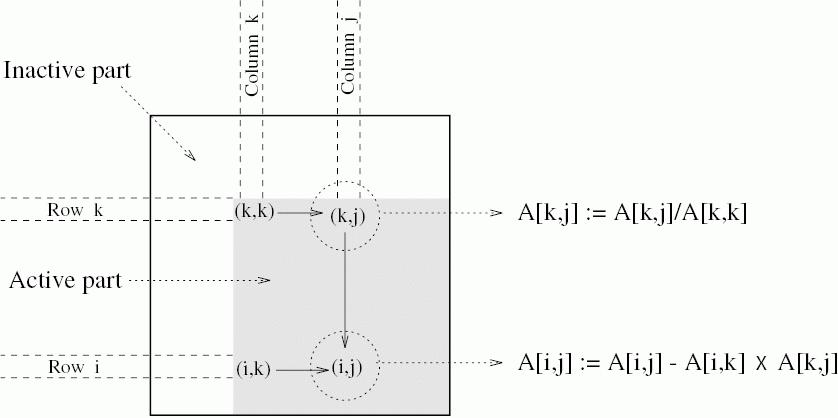
\includegraphics[width=\textwidth]{gauss-alg.jpg}

\begin{breakablealgorithm}
  \caption{普通高斯消元算法伪代码}
  \begin{algorithmic}[1] %每行显示行号  
    \Function {LU}{}
    \For {$k:=0$\ \textbf{to}\ $n$}
    \For {$j:=k+1$\ \textbf{to}\ $n$}
    \State {$A[k,j]:=A[k,j]/A[k,k]$}
    \EndFor
    \State{$A[k,k]:=1.0$}
    \For {$i:=k+1$\ \textbf{to}\ $n$}
    \For {$j:=k+1$\ \textbf{to}\ $n$}
    \State {$A[i,j]:=A[i,j]-A[i,k]*A[k,j]$}
    \EndFor
    \State{$A[i,k]:=0$}
    \EndFor
    \EndFor
    \EndFunction
  \end{algorithmic}
\end{breakablealgorithm}

观察高斯消去算法,注意到伪代码第 4,5 行第一个内嵌循环中的
A[k, j] := A[k, j] / A[k, k] 以及伪代码第 8、9、10 行双层 for 循环中的
A[i, j] := A[i, j] - A[i, k] * A[k, j] 都是可以进行向量化的循环。可以通过
SIMD 扩展指令对这两步进行并行优化。

\subsection{消元子模式的高斯消元算法}
本算法源自布尔 Gröbner 基计算。
Gröbner基是一种广泛应用于复杂高次方程体系的计算方法,它是 Buchberger首先提出的。它的实质是从多项式环的任何一个理想的生成元上,对一组“好的”生成元进行描述和计算,从而对理想的构造进行分析,并对其进行一些理想的运算。由于数学、科学和工程学中的许多问题都可以用多元多项式方程组表示(例如,理想,模块和矩阵),Gröbner基的代数算法在理论物理学、应用科学和工程学中具有广泛的应用。
在 HFE80 的 Gröbner 基计算过程中,高斯消元时间占比可以达到90\% 以上。考虑到此算法中高斯消元的特殊性,为加快高斯消元速度,设计此算法。
\subsubsection{符号说明}
$R$:所有消元子构成的集合

$R[i]$:首项为 $i$ 的消元子

$E$:所有被消元行构成的数组

$E[i]$:第 $i$ 个被消元行

$lp(E[i])$:被消元行第 $i$ 行的首项

这里首项的含义:首项是指某行下标最大的非零项的下标,如某行为 011000,从左到右下标分别为 5,4,3,2,1,0,那么首项为 4,因为该行非零项下标为 3,4,其中最大值为 4。

\subsubsection{算法伪代码}
\begin{breakablealgorithm}
  \caption{串行算法伪代码}
  \begin{algorithmic}[1] %每行显示行号  
    \Function {Gauss}{}
    \For {$i:=0$\ \textbf{to}\ $m-1$}
    \While {$E[i]!=0$}
    \If{$R[lp(E[i])]!=NULL$}
    \State $E[i]:=E[i]−R[lp(E[i])]$
    \Else\State{$R[lp(E[i])]:=E[i]$}
    \State\textbf{break}
    \EndIf
    \EndWhile
    \EndFor
    \State \Return{$E$}
    \EndFunction
  \end{algorithmic}
\end{breakablealgorithm}

在这里,最外层循环代表了对每一个被消元的行的遍历。内层循环代表每一条被消元行,若行没有被消为0,则按照其第一项选择消元;如果有适当的消元符,则用该消元子消元,或者将该被消元行作为消元子,参加下一步的高斯消元。
并行算法内容由串行算法改进。

\section{背景知识}

\subsection{数据结构}

可采用位向量方式存储每个消元子和被消元行,优点是消元操作变为位向量异或操作,算法实现简单,且适合并行化,易达到更高的并行效率,缺点是 Gröbner 基计算中产生的消元子和被消元行非常稀疏,非零元素( 1 元素)在 5 \% 以下,位向量存储和计算可能并非最优。
也可采用类似倒排链表的存储及方式——可认为是稀疏 0 / 1 矩阵的紧凑存储方式,每个消元子和被消元行只保存1元素的位置,且按升序排列,从而类似倒排链表数据结构。优点是存储空间占用更少,缺点是算法设计更复杂,并行化难度高。

\subsection{数据访问}

矩阵规模可能非常庞大,达到数百万行 / 列,难以全部放入内存。此时,需要设计的是外存算法,考虑如何分批次将数据读入内存进行处理,同时又保证正确性。对外存算法,算法分析和时间测试除了考虑计算之外,还要考虑 I / O 时间。

\subsection{并行化方法}

\begin{enumerate}
  \item 对位向量存储方式,两行间消元操作的并行化很直接,无论 SIMD、多线程还是 MPI、GPU,将向量拆分,子向量的异或即自然形成任务,可分配给不同的计算单元。当矩阵规模大到百万级别时,采取这种并行方式就够了。但当矩阵规模没有那么大时,一个消元操作计算量不足以支撑较大规模并行,就需要考虑消元操作间的并行,设计适合的并行任务划分,在提高并发度的同时保证正确性。
  \item 对类倒排链表存储方式,可以考虑循环展开和多线程优化。
  \item 当矩阵规模非常庞大,需使用外存算法时就要同时考虑计算和访存。多线程并行化时可考虑计算和访存异步模式,在前台线程进行消元计算时、后台线程读取下一步要处理的数据,这需要仔细设计计算和 I / O 步骤,降低依赖关系,以便实现异步模式。
\end{enumerate}

\section{研究计划}

本课题的研究由丁屹和卢麒萱共同完成,具体两人的分工如下:

\begin{itemize}
  \item 丁屹负责尝试将高斯消元算法在 arm 平台使用 SIMD、Pthread、OpenMPI 等框架加速,使用 NVIDIA 的 CUDA 框架加速,在各个平台运行测试并对结果进行性能分析对比。
  \item 卢麒萱负责在本机 (Arch Linux x86) 平台实现普通的和特殊的串行高斯消元算法,使用 SIMD、Pthread、OpenMPI 等框架加速并提前测试,并编写测试代码、尝试结合多种加速方法。
\end{itemize}

\newpage

\section{参考文献}
\cite{1}\cite{2}

\bibliographystyle{plain}
\bibliography{Parallel-Programming-2.bib}

\end{document}